\subsection{Thermal Simulations} \label{compvis_thermalsims}

    This section describes the thermal simulations, which aim to investigate the detectability of a landmine in challenging environmental conditions with a thermal sensor.
    
    \subsubsection{Physical Principles} \label{physical_principles}
    
         \noindent The transient thermal behaviour of the soil and a buried mine is described by the heat equation. For a domain with \textbf{piecewise constant properties}, the heat equation can be written as
        
        \begin{equation} \label{heat_eqn}
            \frac{\partial T}{\partial t} = \alpha \nabla^2 T, \quad \text{where} \quad \alpha = \frac{k}{\rho c_p}.
        \end{equation}
    
        \noindent \( T \) (K) is the temperature, \( t \) (s) is time, \( \alpha \) (m$^2$/s) is the thermal diffusivity, \( k \) (W/m·K) is the thermal conductivity, \( \rho \) (kg/m$^3$) is the mass density, and \( c_p \) (J/kg·K) is the specific heat capacity. It should be noted that \(\alpha\) is the only material property present in the governing equation for conductive heat transfer in the soil. This means that the only way that a \textit{buried} landmine can have any effect on the temperature field in the soil, and thus be detected by a thermal sensor, is if \(\alpha_{\text{mine}} \neq \alpha_{\text{soil}} \).
    
        The temperature field will always satisfy Equation \ref{heat_eqn}, but the specific temperature distribution in, and on the surface of the soil (which determines the infrared return to the sensor), is governed by the boundary conditions. The boundary conditions are dictated by different mechanisms of heat transfer, which are: \label{sec:cv_architecture_comparison} heat transfer between the air and the soil, \label{sec:cv_architecture_comparison} in the soil, and radiation, which includes \label{sec:cv_architecture_comparison} from sun and sky incident on the soil, and black-body \label{sec:cv_architecture_comparison} from the soil surface. These must all be accurately modelled to faithfully represent the soil temperature distribution. It is also noted that when mines are buried, the soil is overturned. This disturbance can increase the thermal contrast on the soil surface, but is not modelled here.
            
    
    \subsubsection{Details of the Solver}
    
        The solver is a finite element solver implemented in MATLAB. The thermal model simulates heat conduction in a two-dimensional soil domain of dimensions $L =1$\,m $H = 1$\,m. The domain is defined as a rectangular region $\Omega_1$ representing the soil, with a circular inclusion $\Omega_2$ embedded within it to simulate the presence of a buried landmine. The mine is modelled as a circle with \(d=0.1\,\text{m}\) with \(h=0.9\,\text{m}\), which corresponds to a typical burial depth of 10\,cm. A finite element mesh is generated over the domain using MATLAB's \texttt{generateMesh()} function. For the final high-resolution simulations a maximum mesh size of 0.005\,m is used (20 times smaller than the diameter of the mine), while a coarser mesh (maximum element size 0.02\,m) is used during the iterative initial condition refinement in Section \ref{sec:cv_initial_conditions}. A mesh convergence study was conducted by lowering the maximum mesh size and observing no significant change in the peak temperature difference above the landmine for the high-resolution mesh.
        
        The transient heat conduction problem is solved using the Finite Element Method (FEM) with triangular linear Lagrange (P1) elements to discretise the spatial domain. The time-dependent heat equation is integrated using an implicit backward Euler scheme. MATLAB's PDE Toolbox automatically solves the systems of equations with a sparse direct solver \footnote{\url{https://uk.mathworks.com/help/matlab/math/partial-differential-equations.html}}.
    
         \begin{figure}[htbp]
          \centering
          \begin{subfigure}[t]{0.48\textwidth} % Top-aligned subfigures
            \centering
            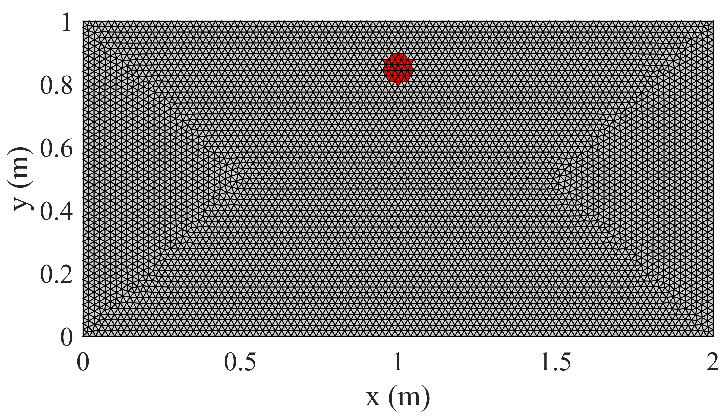
\includegraphics[width=\textwidth]{figs/Rory/thermal_mesh_new.pdf}
            \caption{Coarse mesh visualization}
            \label{fig:thermal_mesh}
          \end{subfigure}
          \hfill
          \begin{subfigure}[t]{0.48\textwidth}
            \centering
            \raisebox{2.5mm}{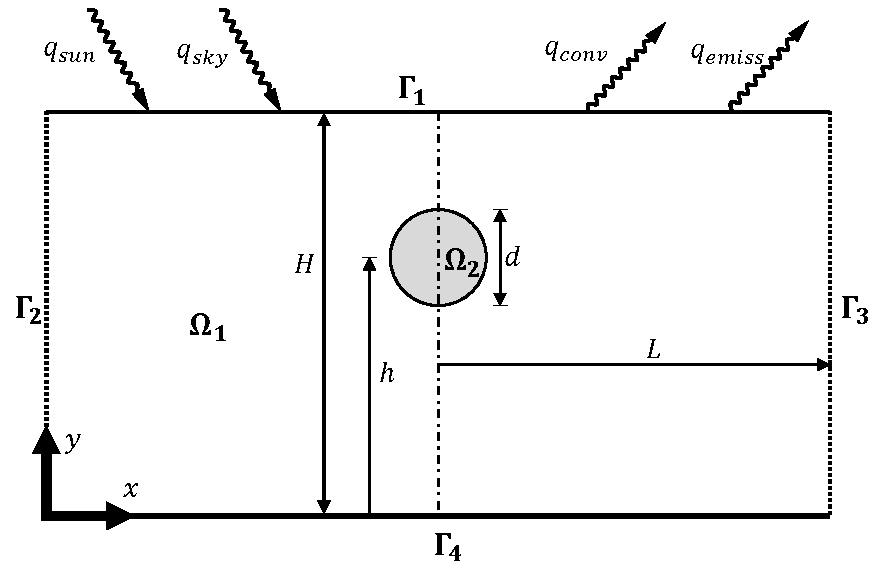
\includegraphics[width=\textwidth]{figs/Rory/thermal_domain.pdf}}
            \caption{Domain configuration}
            \label{fig:thermal_domain}
          \end{subfigure}
          \caption[Thermal simulations setup]{Thermal simulation setup: (a) 4× downsampled mesh (max element size 0.02\,m vs. 0.005\,m resolution used in simulations), landmine shown in red; (b) Numerical domain with soil region ($\Omega_1$), mine inclusion ($\Omega_2$), boundary labels ($\Gamma_1$\--$\Gamma_4$), and heat flux components ($q_i$).}
          \label{fig:thermal_setup}
        \end{figure}
    
    \subsubsection{Boundary Conditions} 
    
        The bottom boundary of the domain, $\Gamma_4$, is modelled as an isothermal Dirichlet condition, with the deep soil temperature set to average air temperature $T_{\infty}$, which approximates the thermal inertia of the soil. The left and right boundaries, $\Gamma_2$, $\Gamma_3$,  are modelled as adiabatic (zero heat flux) to prevent lateral heat exchange. This represents a symmetry condition, where lateral landmines are equally spaced. The top boundary, $\Gamma_1$,  is subject to a time-dependent Neumann boundary condition that accounts for:
    
        \begin{itemize}
        
            \item \textbf{Solar Insolation:} A periodic function models the diurnal variation of solar radiation for a given location and time of year. The solar flux,  $\dot{q}_{sun}$  (W/m$^2$), is modelled using solar insolation data for Afghanistan\footnote{\url{https://www.pveducation.org/pvcdrom/properties-of-sunlight/calculation-of-solar-insolation}} (Kabul) on June 5th.
            
            \item \textbf{Convection:} Heat exchange with the ambient air is governed by convection, with the heat flux dependent on the wind speed, and the temperature difference between the soil surface and the ambient air. A low-order correlation based model was used to model convection, suggested by Kahle et al. \cite{kahle1997model}: $\dot{q}_{conv} \approx \rho c_p C_D(w+2)(T - T_{\infty})$, where \(C_D\)(-) is the drag coefficient of the soil and taken as 0.02, \(w\) (m/s) is the average wind speed, and \(T_\infty\) (K) is the ambient air temperature.
            
            \item \textbf{Irradiance from the Sky:} Downward radiation from the sky is modelled using an empirical relation in Nguyen et al. \cite{nguyen2008inverse}: $\dot{q}_{\text{sky}} = T_{\infty} \left( 0.61 + 0.05 \sqrt{\omega} \right)^{0.25}$, where \(\omega\) (mmHg) is the water vapour pressure, and is taken as 760\,mmHg.
            
            \item \textbf{Radiative Emission:} Radiation emission is modelled using the Stefan-Boltzmann law \footnote{\url{https://en.wikipedia.org/wiki/Stefan–Boltzmann_law}}: $\dot{q}_{emiss} \approx \epsilon \sigma T^4$, where \(\epsilon\) (-) is the emissivity coefficient taken as 0.9 (suggested in Nguyen et al.), and \(\sigma\) (W/(m$^2$·K$^4$)) is the Stefan–Boltzmann constant .
            
        \end{itemize}
    
        \noindent The \textbf{net heat flux leaving the soil} is given by the location dependant Neumann boundary condition on $\Gamma_1$:
        \begin{equation}
        \dot{q}_{net} = \epsilon \sigma T^4+ \rho c_p C_D(w+2)(T - T_{\infty}) - T_{\infty} \left( 0.61 + 0.05 \sqrt{\omega} \right)^{0.25}  - \dot{q}_{sun}
        \end{equation}
        
    \subsubsection{Initial Conditions} \label{sec:cv_initial_conditions}

        \noindent The thermal field of the domain is initialised as homogeneous at the deep soil temperature $T_{\infty}$. A coarse resolution simulation (using a 0.02\,m element size) is first run for a 24-hour period, and the \textbf{thermal field at the final time step is saved, and used as the initial condition for a subsequent, similar simulation}. This process is iterated until the average temperature at the surface after 24 hours converges to within a tolerance of 0.01\,$^{\circ}$C. The converged temperature distribution at 24 hours is used as the initial condition for a 24 hour high-resolution simulation with 0.005\,m element size. This approach to set up the initial conditions ensures that the \textbf{temperature field is 24-hour periodic} given 24-hour periodic boundary conditions. The converged initial condition for Afghanistan conditions is visualised in Figure \ref{fig:combined_thermal}, with the surface temperature distribution also plotted for clarity.

    \subsubsection{Simulation Setup for Afghanistan} \label{thermal_setup}
    
        For this study, the simulation is set up to replicate extreme environmental conditions found in Afghanistan. The solar insolation function is configured for a latitude of 33\(^\circ\) and conditions on 15th June, a month with almost no rainfall, to ensure constant soil parameters. The wind speed is set at 4\,m/s. These represent the most difficult environmental conditions for thermal detection. Most landmines contain little to no metal—apart from the firing pin—and are primarily composed of high explosives very similar in composition to TNT \cite{szymanik2011soil}. Therefore, the mine thermal properties are the properties of TNT. This aspect is discussed in Section \ref{landmines}. Table \ref{tab:properties} lists the simulation parameters used for the thermal simulation.
    
        \begin{table}[ht]
        \centering
        \caption{Simulation Parameters}
        \label{tab:properties}
        \begin{tabular}{lccc}
        \hline
        \textbf{Parameter} & \textbf{Value} & \textbf{Units} & \textbf{Comments}\\
        \hline
        Mine Diameter \(d\)       & 0.1     & m    & Typical\\
        Mine Depth \(h\)          & 0.1   & m    & Typical\\
        Soil Thermal Conductivity $k_{\Omega_1}$ & 2  & W/(m$\cdot$K) & \cite{szymanik2011soil}\\
        Soil Density $\rho_{\Omega_1}$     & 1900     & kg/m$^3$ & \cite{szymanik2011soil}\\
        Soil Specific Heat Capacity $c_{p,{\Omega_1}}$  & 1480     & J/(kg$\cdot$K) & \cite{szymanik2011soil}\\
        Soil Thermal Diffusivity $\alpha_{\Omega_1}$ & $0.711$ & mm$^2$/s    & Equation \ref{heat_eqn}\\
        Mine Thermal Conductivity $k_{\Omega_2}$ & 0.25  & W/(m$\cdot$K) & \cite{szymanik2011soil}\\
        Mine Density $\rho_{\Omega_2}$      & 1140     & kg/m$^3$ & \cite{szymanik2011soil}\\
        Mine Specific Heat Capacity $c_{p,{\Omega_2}}$ & 1980     & J/(kg$\cdot$K) & \cite{szymanik2011soil}\\
        Mine Thermal Diffusivity $\alpha_{\Omega_2}$ & 0.111 & mm$^2$/s    & Equation \ref{heat_eqn}\\
        Wind Speed \(w\)          & 4      & m/s  & Typical for June \tablefootnote{\url{https://weather-and-climate.com/average-monthly-Wind-speed,Kabul,Afghanistan}}\\
        \hline
        \end{tabular}
        \end{table}

   


    \subsubsection{Results and Validation} \label{Results and Validation}
    
         The simulation showed that the peak \(\Delta T\) was 1.7\,K, at a time of just past 12:30 (Afghan local time), and sustained a \(\Delta T \geq 1\)\,K for over 7 hours (from around 10:00 to 17:30). Given that the sensitivity of the thermal sensor is 0.05\,K (Section \ref{sensor_overview}), these results show that for a large period of the day, \(\Delta T\) is more than 20$\times$ the sensitivity of the sensor, and thus, by the detectability hypothesis, \textbf{landmines can be readily detected}. As discussed earlier in this section, the thermal sensor will work even better than this in other environments, because Afghanistan represents a challenging environmental condition for thermal detection.
    
        \begin{figure}[htbp]
            \centering
            \begin{minipage}[b]{0.48\textwidth} % Adjust width as needed
                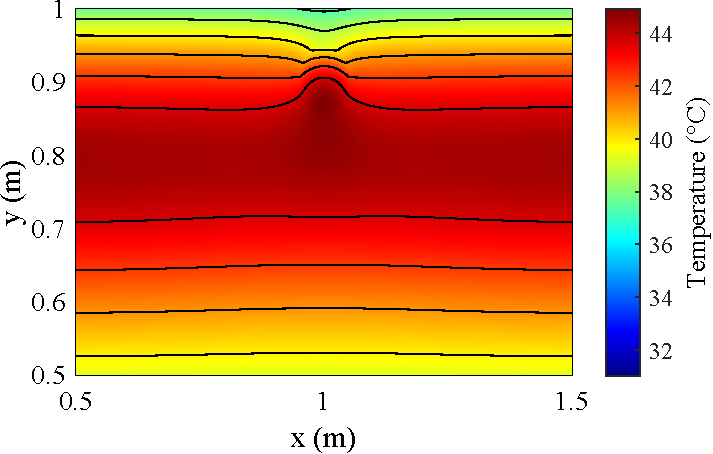
\includegraphics[width=\textwidth]{figs/Rory/A_temp_distribution.pdf}
                %\caption{Enlarged simulation domain at local Afghanistan time midnight} % Remove individual caption
                %\label{fig:thermal_result} % Remove individual label
            \end{minipage}
            \hfill % Add horizontal space between the figures
            \begin{minipage}[b]{0.48\textwidth} % Adjust width as needed
                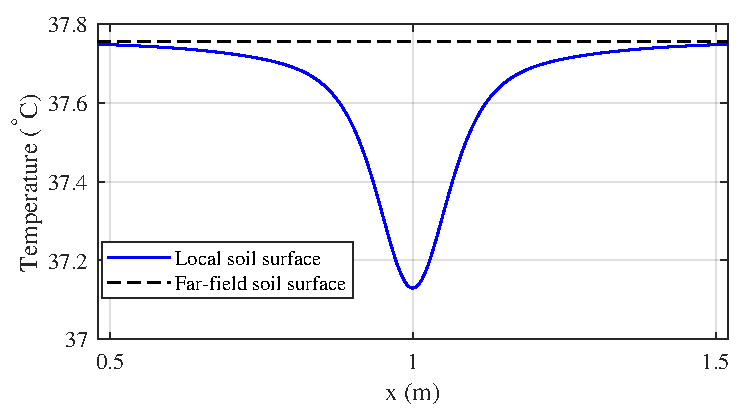
\includegraphics[width=\textwidth]{figs/Rory/1D_distribution_cropped.pdf}
                %\caption{Surface distribution} % Remove individual caption
                %\label{fig:thermal_1D} % Remove individual label
            \end{minipage}
            \caption[Converged initial condition]{\textbf{Left:} Converged initial condition plotted both as a 2D contour plot of a zoomed section of the domain. \textbf{Right:} A 1D line plot of the surface distribution over the same x-axis.}
            \label{fig:combined_thermal}
        \end{figure}

    \subsubsection{Sensitivity Analysis} \label{sec:cv_sensitivity}
    
        \paragraph{Motivation}
            
            \noindent A key parameter with uncertainty is the soil thermal conductivity. Soil conductivity can be hard to measure accurately, has high spatial variability, and fluctuates over short time-spans due to precipitation and evaporation. Moreover, for fuzzy rule definition (Section \ref{fuzzy_rules}), the influence of varying soil conductivity on \(\Delta T\), is not immediately obvious. Therefore, a dedicated sensitivity study is important to quantify how changes in soil conductivity affect \(\Delta T\).
        
        \paragraph{Study}
        
            \noindent For each value of soil conductivity between 0.2\,W/mK and 3.6\,W/mK, with even spacing of 0.2\,W/mK, a high-resolution thermal simulation was run (as described earlier in this section), with all other simulation parameters unchanged from in Table \ref{tab:properties}. The peak \(\Delta T\) over the course of one day was recorded for each simulation.
            
            As illustrated in Figure \ref{fig:conductivity}, the peak \(\Delta T\) increases with soil conductivity beyond approximately 0.4 W/mK. This threshold corresponds to the point where the thermal diffusivity of the soil matches that of the mine, rendering the mine thermally ‘invisible’—since thermal diffusivity is the sole mechanism through which the mine influences the temperature field, as discussed in Section \ref{physical_principles}. Linearisation of the thermal conductivity response at an operating point of 2\,W/mK, representative of Afghanistan conditions, indicates that the peak \(\Delta T\) value has a slope of approximately 0.175 K (W/mK)$^{-1}$. Assuming natural variation in soil thermal conductivity of less than 50\% of its nominal value, the expected variation in peak \(\Delta T\) is on the order of 0.1\,K. This fluctuation is an order of magnitude lower than the peak \(\Delta T\) simulated with Afghanistan conditions, and just 3 times the sensitivity of the thermal sensor \ref{sensor_overview}. Thus peak \(\Delta T\) is insensitive to soil thermal conductivity. Note the upwards trend for peak \(\Delta T\) with soil thermal conductivity greater than 0.4 W/mK, a result used in Section \ref{fuzzy_rules}.

        
        Interestingly, this result is in contrast to that described in Alqudsi et al. \cite{alqudsi2021review}, who suppose that detection of landmines with infrared sensors becomes more difficult as the soil becomes wetter.

        \begin{figure}
            \centering
            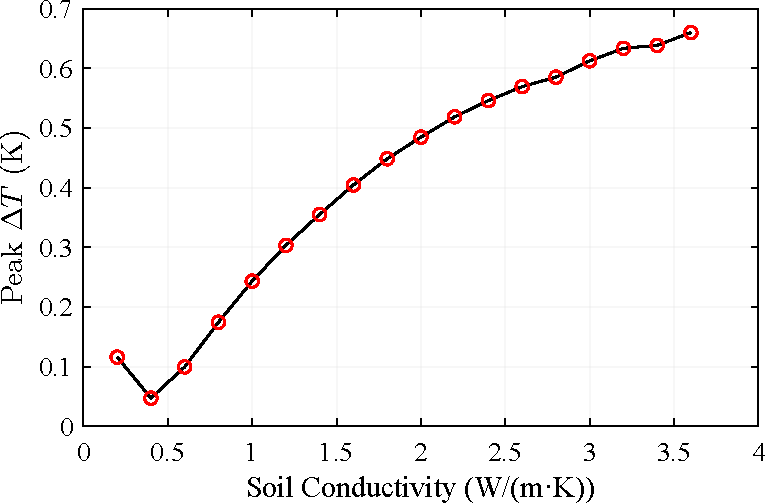
\includegraphics[width=0.48\textwidth]{figs/Rory/thermal_sensitivity_conductivity.pdf}
            \caption[Effect of soil conductivity on the peak $\Delta T$ over a 24-hour period]{Effect of soil conductivity on the peak $\Delta T$ over a 24-hour period. The inversion point near 0.4 W/mK is evident.}
            \label{fig:conductivity}
        \end{figure}
        